\chapter{System V File System}
\label{s5fs}

\section{Introduction}

The System V File System, or ``S5FS,'' is a file system based on the original Unix file system.  Although it lacks some of the complex features of a modern file system, Weenix uses it because it provides an excellent introduction to the issues involved in writing an on-disk file system.

In completing the S5FS assignment, you will provide its implementation for the full VFS interface.  You will come across many different S5FS objects that interact with each other.  Most of these object types are on-disk data structures -- that is, the memory they occupy is actually being saved to disk (the only S5FS type which is not backed by disk is the struct representing the file system itself).

Remember to turn the \texttt{S5FS} project on in \texttt{Config.mk} and \texttt{make clean} your project before you try to run your changes.
\section{Disk Layout}

% picture of S5FS disk layout
\begin{figure}
    \centering
    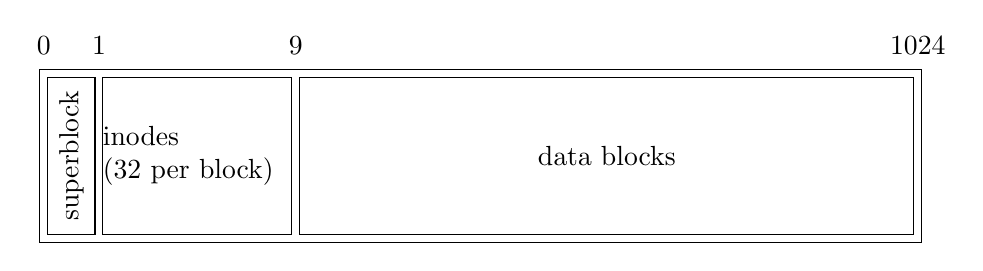
\begin{tikzpicture}
        % labels for disk block numbers and the bounding box
        \draw (-0.05,2.4) node {0};
        \draw (.65,2.4)   node {1};
        \draw (3.15,2.4)  node {9};
        \draw (11.05,2.4) node {1024};
        \draw (-.1,-.1)   rectangle (11.1,2.1);
        % the superblock box
        \draw (0,0)   rectangle (.6,2);
        \draw (.3,1)  node[rotate around={90:(0,0)}] {superblock};
        % the inodes box
        \draw (.7,0)  rectangle (3.1,2);
            % TODO centering text with align=center
        \draw (1.9,1) node[text width=2.4cm] {inodes\\(32 per block)};
        % the data blocks box
        \draw (3.2,0) rectangle (11,2);
        \draw (7.1,1) node {data blocks};
    \end{tikzpicture}
    \caption{The default disk layout for Weenix.}
\end{figure}

\subsection{Superblock}

The first block of the disk (block number zero) is called the superblock, which contains metadata about the file system. The important data fields inside it are the inode number of the root directory, the number of the first free inode, the first section of the free block list, the number of free blocks currently referenced in that section of the free block list, and the total number of inodes in use by the filesystem. The less important fields are the ``magic number'' for S5FS disks (used as a sanity check for the OS to determine that the disk you are reading is formatted as an S5FS disk), and the version number of S5FS we are using. The in-memory copy of the superblock is stored in a \texttt{s5\_super\_t} struct. For more information about the structure of the free block list, check out the section on \wlink{datablocks}{data blocks} below.

\subsection{Inodes}

Next, there is an array containing all the inodes for the file system. Each inode requires 128 bytes of space, and each disk block is 4096 bytes, so we store 32 inodes per block. Inodes are referred to by their index in the array, and are stored in memory as \texttt{s5\_inode\_t} structs.  Each inode is either free, or it corresponds to some file in the file system.

If an inode is not free, it represents a file presently on disk.  The inode holds of the size of the file, the type of the file (whether it is a directory, character device, block device, or a regular file), the number of links to the file from other locations in the file system, and where the data blocks of the file are stored on disk.

If an inode is free, it need only be marked as empty and contain the inode number of the next free inode in the free list (or \texttt{-1} if it is the last element in the list). This link is stored in the \texttt{s5\_freesize} field (you can think of that field as being a \texttt{union} whose interpretation depends on whether the inode is free or not).

The link count on an inode has a slightly different meaning based on whether or not Weenix is currently running. If Weenix is shut down, the link count simply reflects the number of directory entries which point to this file. However, while the OS is running, calling \texttt{vget()} on some file for the first time will result in a call to S5FS's implementation of \texttt{read\_vnode()}, which will increment the link count of the inode by one as long as the file is referenced by a vnode. Note that the link count will only be incremented when the file is first read from disk, not every time \texttt{vget()} is called on that file. Once the vnode's reference count drops to zero, the call to \texttt{vput()} will call S5FS's implementation of the \texttt{delete\_vnode()} function, which will decrement the link count of the inode. This extra link count is used to prevent the inode from being deleted from disk as long as some vnode still references it (even if the file has been unlinked from disk) so that any process that is using the file should have no problem reading it. As such, the link count for a new file should be two: one link from its parent directory and one from Weenix. Note that this is slightly different for directories; see the section on \wlink{directories}{directories} for details.

As mentioned above, the location of the data blocks for a file are also stored in the inode for the file. The inode itself keeps track of \texttt{S5\_NDIRECT\_BLOCKS} data block numbers directly, but this is not usually enough for a large-ish file. Luckily, S5FS inodes for ``large'' files also contain a pointer to an indirect block, which is a disk block filled with more data block numbers (in case it isn't clear: by ``pointer'' in this context we mean a disk block number, not a memory address). It is able to store up to \texttt{S5\_BLOCK\_SIZE / sizeof(int)} more block numbers. In a production file system, you should be able to support arbitrarily long files, which would require arbitrarily long indirect block chains (or, more likely, B-trees), but in Weenix we choose to only implement a single indirect block for simplicity. This means that there is a maximum file size; make sure you handle this error case correctly.

% picture of inode, indirect block, data blocks
\begin{figure}
    \centering
    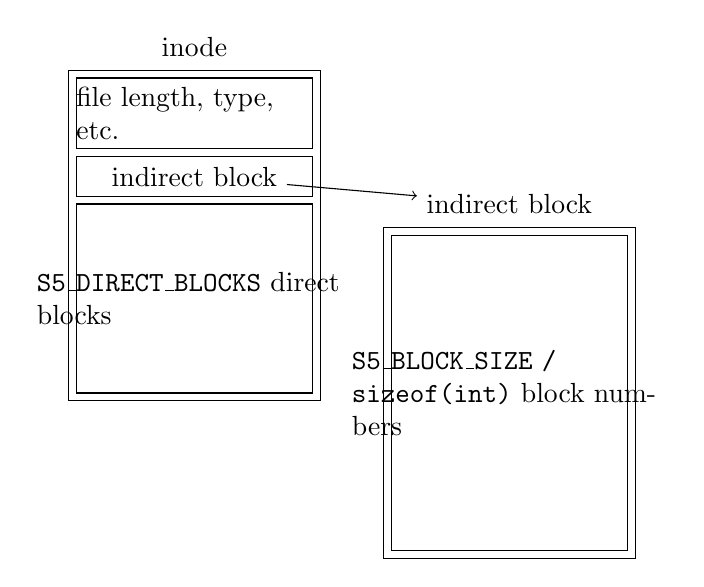
\begin{tikzpicture}
        % the inode label and bounding box
        \draw (1.5,4.4) node {inode};
        \draw (-.1,-.1) rectangle (3.1,4.1);
        % first data fields
        \draw (0,3.1) rectangle (3,4);
            % TODO centering text with align=center
        \draw (1.5,3.55) node[text width=3cm] {file length, type, etc.};
        % the indirect block label
        \draw (0,2.5) rectangle (3,3);
        \draw (1.5,2.75) node (indirect-pointer) {indirect block};
        % the direct blocks
        \draw (0,0) rectangle (3,2.4);
            % TODO centering text with align=center
        \draw (1.5,1.2) node[text width=4cm] {\texttt{S5\_DIRECT\_BLOCKS} direct blocks};
        
        % the indirect block
        \draw (3.9,-2.1) rectangle (7.1,2.1);
        \draw (5.5,2.4) node (indirect-block) {indirect block};
        \draw (4,-2) rectangle (7,2);
            % TODO centering text with align=center
        \draw (5.5,0) node[text width=4cm] {\texttt{S5\_BLOCK\_SIZE /\\sizeof(int)} block numbers};
        
        % arrow to indirect block
        \draw [->] (indirect-pointer) -- (indirect-block);
    \end{tikzpicture}
    \caption{An inode with an indirect block (data blocks not pictured).}
\end{figure}

While the default disk size gives you space for several hundred data blocks, the indirect block will allow a single file to use thousands of blocks. This might seem unnecessary, however it allows for the implementation of sparse files. If a file has a big chunk of zeros in it, Weenix will not waste actual space on the disk to represent them; it just sets the block index to zero. When reading a file, if a block number of zero is encountered, then that entire block should consist of zeroes. Remember that zero is guaranteed to be an invalid data block number because it is the block number of the superblock.

\subsection{Data Blocks} \label{datablocks}

Data blocks are where actual file contents are stored. They occur on disk after the inode array and fill the remainder of the disk. For simplicity, disk blocks and virtual memory pages are the same number of bytes in Weenix, although this is not necessarily true for other operating systems.

The contents of the data blocks are obviously dependent on what file they are filled with (except for directories, which also use data blocks but have a special format described below) unless they are in the free block list. Instead of a free list where each link only points to one more link, which would be wildly inefficient due to frequent seek delays, S5FS uses a list where each link in the list contains the numbers of many free blocks, the last of which points to the next link in the free list. The first segment of the free list is stored in the superblock, where up to \texttt{S5\_NBLKS\_PER\_FNODE} blocks are stored. The last element of this array is a pointer to a block containing \texttt{S5\_NBLKS\_PER\_FNODE} more free blocks, the last of which is a pointer to a block with more free pointers, and so on. The last free block in the list has a \texttt{-1} in the last position to indicate there are no more free blocks. After the second-to-last free block in the superblock's array is used, the next set of free blocks should be copied out of the next block, and then the block they were just copied from can be returned as the next free page.

% picture of free block list
\begin{figure}
    \centering
    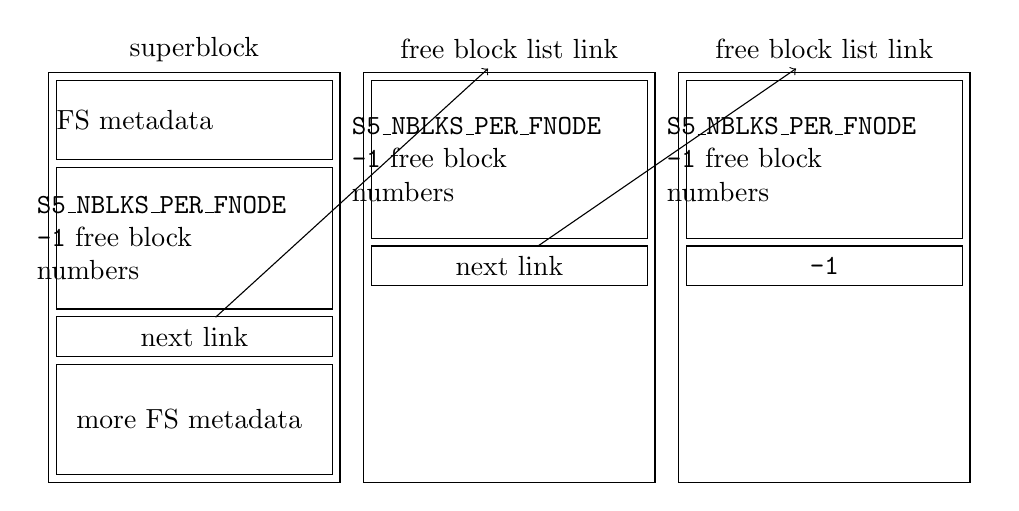
\begin{tikzpicture}
        % the inode label and bounding box
        \draw (1.75,5.4) node {superblock};
        \draw (-.1,-.1) rectangle (3.6,5.1);
        % first data fields
        \draw (0,4.0) rectangle (3.5,5);
            % TODO centering text with align=center
        \draw (1.75,4.5) node[text width=3.5cm] {FS metadata};
        % the direct blocks
        \draw (0,2.1) rectangle (3.5,3.9);
            % TODO centering text with align=center
        \draw (1.75,3) node[text width=4cm] {\texttt{S5\_NBLKS\_PER\_FNODE\\-1} free block\\numbers};
        % the next label
        \draw (0,1.5) rectangle (3.5,2);
        \draw (1.75,1.75) node (next-pointer) {next link};
        % other data fields
        \draw (0,0) rectangle (3.5,1.4);
            % TODO centering text with align=center
        \draw (1.75,.7) node[text width=3cm] {more FS metadata};
        
        % the next free block
        \draw (3.9,-.1) rectangle (7.6,5.1);
        \draw (5.75,5.4) node (next) {free block list link};
        \draw (4,3) rectangle (7.5,5);
            % TODO centering text with align=center
        \draw (5.75,4) node[text width=4cm] {\texttt{S5\_NBLKS\_PER\_FNODE\\-1} free block\\numbers};
        % the next label
        \draw (4,2.4) rectangle (7.5,2.9);
        \draw (5.75,2.65) node (next-next-pointer) {next link};
        
        % the next free block
        \draw (7.9,-.1) rectangle (11.6,5.1);
        \draw (9.75,5.4) node (next-next) {free block list link};
        \draw (8,3) rectangle (11.5,5);
            % TODO centering text with align=center
        \draw (9.75,4) node[text width=4cm] {\texttt{S5\_NBLKS\_PER\_FNODE\\-1} free block\\numbers};
        % the next label
        \draw (8,2.4) rectangle (11.5,2.9);
        \draw (9.75,2.65) node {\texttt{-1}};
        
        % arrow to next block
        \draw [->] (next-pointer) -- (next);
        
        % arrow to next-next block
        \draw [->] (next-next-pointer) -- (next-next);
    \end{tikzpicture}
    \caption{The free block list.}
\end{figure}

\subsection{Directories} \label{directories}

S5FS implements directories as normal files that have a special format for their data. The data stored in directory files is essentially just a big array of pairs of inode numbers and the filenames corresponding to those inode numbers. Filenames in S5FS are null-terminated strings of length less than or equal to \texttt{S5\_NAME\_LEN} (including the null character). Any entry with a zero-length name indicates an empty or deleted entry. Note that every directory contains one entry for ``\texttt{.}'' and one for ``\texttt{..}'', corresponding to the current directory and the parent directory, respectively, from the beginning of its existence to the moment it is deleted. The link count for a newly-created directory should be two (one reference from its parent directory, and one from the running copy of Weenix that just created it). The convention for weenix is that the self-reference from a directory to itself (\texttt{.}) is \emph{not} counted towards the link count.

\section{Caching}

At this point, you know a lot about how the on-disk filesystem looks and could probably inspect the disk block-by-block and understand what files are stored there. However, while working on this part of Weenix, you will not need to directly read and write from the disk, even in the most low-level functions. Instead, you will use the VM caching system to read blocks from disk into memory. You can then manipulate these pages in memory, and the pageout daemon will automatically handle writing them back to disk.

The Weenix caching system uses two different types of objects: page frames, which are each responsible for tracking one page/block of data, and memory objects, which are each associated with a number of page frames that hold the data for that memory object. In the codebase, the names for these objects are \texttt{pframe\_t}s and \texttt{mmobj\_t}s, respectively. Each memory object represents some data source, which could be a file, device, or virtual memory region. This means that page frames are used to reference the blocks of files, blocks of a device, and blocks of segments of memory. Specifically, page frames store some metadata about the page they hold and a reference to that page in memory. If a particular page of, say, a file hasn't been paged into memory, there will not yet be a page frame for that page.

To get a particular page frame from a memory object, you should call \texttt{pframe\_get()} on the memory object you wish to get the page from. The data stored in the page is stored at the location pointed to by the page frame's \texttt{pf\_addr} field. When a page frame has been modified, you should mark it as \wlink{pf-states}{dirty} so that it will be cleaned (the changes will be written back to disk) if necessary. The cleaning process uses callbacks in the disk's memory object to write the data back to disk.

To use an inode from disk, you must get its page from the disk memory object (the \texttt{S5\_INODE\_BLOCK()} macro will tell you which disk block to get) and then use the \texttt{S5\_INODE\_OFFSET()} macro to index into the page. When you are changing a file or the filesystem data structures, make sure that you remember to dirty the indirect block, inode, and superblock if necessary. Note the presence of the \texttt{s5\_dirty\_inode()} and \texttt{s5\_dirty\_super()} calls for this purpose. Remember that you should never clean pages yourself as either the pageout daemon or the Weenix shutdown sequence will take care of that automatically.

While working on S5FS, you may notice that there are two very similar methods for accessing the data on disk: calling \texttt{pframe\_get()} on the memory object for the block device (the disk) and on the memory object for the file. Therefore, it can sometimes be confusing which one to use. Although this may sound like common sense, it is important that you use a file's memory object every time you are dealing with a file, and use the block device's memory object when you are implementing pieces of the filesystem that are ``low-level enough'' to know how a file is split across multiple blocks on disk. If you accidentally use the disk memory object instead of the file memory object, you will be short-circuiting a couple layers of abstraction that will be necessary later on.

\subsection{Page Frame States} \label{pf-states}

As alluded to above, there are several states which a page frame can be in. At boot time, all page frames are \emph{free}, meaning they are waiting to be allocated. Some of the page frames will eventually be \emph{allocated}, at which point they are added to the allocated page frame list and filled with data. If a change is made inside their associated page of memory, they should be marked as \emph{dirty}.

The allocated page frame list is maintained to ease the implementation of the pageout daemon, which traverses the list and frees page frames and their associated memory pages. Note that any dirty pages will be cleaned (written out to disk) during this step, and non-dirty pages will simply be freed. The pageout daemon should only run when the system is out of memory, although you are allowed to call it other times as well if you choose. However, the use of the pageout daemon raises the question: how will you prevent a page frame from being freed while you are using it?

To solve this potential issue, page frames can also be \emph{pinned} while they are in use. Pages can be pinned multiple times; as long as the pin count of a page frame is greater than zero, it is guaranteed not to be cleaned or freed. This will also be important when you implement virtual memory, since page frames for some types of virtual memory regions will not be backed by disk and can therefore never be safely cleaned or freed. When a page is pinned, it is removed from the allocated frame list and added to the pinned list, and the reverse happens when the last pin is removed.

The only time during S5FS where you should pin pages is when it is possible that your code will block after finding a page frame and before using that frame, since those are the conditions under which the pageout daemon could free the page, causing a memory corruption bug that will be difficult to reproduce. If you are unsure whether some code path might block, it is safer to pin any page frames you are using than not to do so. When you are done using the page frames, make sure you unpin them so that you do not run out of memory.

Finally, to protect page frames from making ill-formed state transitions, page frames can be marked as \emph{busy} while they are in the middle of a state transition. Any concurrent attempts to modify a page frame (not necessarily the page it points to) should block until it is no longer busy.

\subsection{Lazy Cleaning}

One noteworthy feature of Weenix's caching system is that it does not uncache any pages of a file until either the system is out of memory (the pageout daemon may write back some or all of the changes at this point) or Weenix shuts down (the page frame system writes back its changes). This feature was added to improve cache performance for files that are closed and reopened frequently.

Each time \texttt{vput()} is called on a file, the S5FS implementation of \texttt{query\_vnode()} is run to check if the file is still referenced by some directory on disk or some vnode in memory. If it has been deleted from every directory it was present in and you are \texttt{vput()}ing the final memory reference to the file, the blocks of that file that are cached in memory can simply be freed (even if they are dirty) since nobody will ever need to use them again. Otherwise, they are left to be cleaned up at some later point. If you notice that your filesystem is working but none of your changes are being propagated to disk, you may want to check to see if this code path is running.

\section{Error Handling}
\label{S5FS Error Handling}

You always need to check for things that can go wrong. When an error condition occurs, you should return \texttt{-errno} where \texttt{errno} is the error number that indicates the type of error that occurred. For example, if you run out of free data blocks when attempting to write to a new block of a file, you should return \texttt{-ENOSPC}. You should \emph{always} check the return value from non-void functions you call, and if the returned value is negative you often need to propagate it up. Returning \texttt{-1} is not correct.

However, it is also important that your VFS code check for as many errors as possible, so that each file system that it runs need not check the same error cases. If you know that some error condition should always be dealt with at the VFS layer, you should assert that it does not occur in the S5FS layer to identify bugs in your implementation while you develop.

We have tried to indicate some errors that you should check for in the comments, but we have probably not mentioned all of them, so you should go over your code thoroughly to make sure that you handle all possible errors.

\section{Getting Started}

You need to implement:

\begin{itemize}

\item The high-level system calls for S5FS (the VFS interface).  Many of these will have a name such as \texttt{s5fs\_[name]} with a corresponding VFS call named \texttt{do\_[name]}.

\item The low-level subroutines.  These subroutines represent common functionality that may be useful to reuse in many of the high-evel system calls.

\item A few memory management routines (such as \texttt{pframe\_get()}).  This is to understand a little better how the caching system works.

\end{itemize}

\section{Testing}

Your test cases should demonstrate clearly that all functions have been tested properly. While much of the functionality of S5FS will be tested by the tests you used for VFS, there are several cases that may require a bit more thought:

\begin{itemize}
    \item Indirect blocks. (The \texttt{hamlet} file on your virtual disk is provided as an example of a file which needs an indirect block, but don't forget to check the case where you need to allocate one at runtime as well.)
    \item Sparse blocks.
    \item Running out of inodes, data blocks, or file length.
    \item Shutting down and rebooting does not erase your changes.
\end{itemize}

Be sure that your link counts are correct (\texttt{calculate\_refcounts()} will calculate the counts for you). Note that you \emph{must} make sure you are actually shutting down cleanly (i.e. see the ``Weenix halted'' message). Reference count issues will prevent Weenix from shutting down cleanly.

To ease the difficulty of debugging your file system code, we have provided a couple of utilities to help you develop. The \texttt{fsmaker} utility will come in handy for inspecting blocks, inodes, and other data structures on your virtual machine's disk. To read more about how to use \texttt{fsmaker}, run \texttt{fsmaker --help} from the root of your development directory. Your disks are stored in files on the host operating system (the \texttt{user/disk*.img} files), and must be passed to \texttt{fsmaker} as an argument. Also, running the \texttt{./weenix} script with the \texttt{-n} option will create a brand new disk for you and fill it with a bunch of sample files and directories. To begin this assignment, you must use this option at least once, otherwise you will not have a disk to work with.
